% UNIT 1: RATES & PROPORTIONS - LESSON 3 WORKSHEET 2
\documentclass[12pt, letterpaper, fleqn]{article}

% ----------------------------------------------------------
% PACKAGES
% ----------------------------------------------------------
\usepackage{graphicx}
\usepackage{xcolor}
\usepackage[most]{tcolorbox}
\usepackage{amsmath, amssymb}
\usepackage{fancyhdr}
\usepackage[utf8]{inputenc}
\usepackage[T1]{fontenc}
\usepackage{enumitem}
\usepackage{geometry}
\usepackage{tikz}
\usepackage{needspace}
\usepackage{multicol}

\usetikzlibrary{arrows.meta, calc}

% ----------------------------------------------------------
% PAGE SETUP
% ----------------------------------------------------------
\usepackage{times}
\geometry{letterpaper, top=1.25in, bottom=1.25in, marginpar=0.5in}

% ----------------------------------------------------------
% HEADER / FOOTER
% ----------------------------------------------------------
\newcommand{\logowidth}{3cm}
\setlength{\headheight}{20pt}
\setlength{\footskip}{40pt}

\pagestyle{fancy}
\fancyhf{}
\fancyhead[C]{\small\bfseries Equations of Proportional Relationships}
\fancyfoot[L]{\raisebox{2pt}{
\includegraphics[width=\logowidth]{kss.png}}}
\fancyfoot[C]{\thepage}
\fancyfoot[R]{7.3.2}

\renewcommand{\footrulewidth}{0.2pt}

% ----------------------------------------------------------
% THEME COLOR
% ----------------------------------------------------------
\definecolor{customteal}{HTML}{2fbdb9}

% ----------------------------------------------------------
% HELPER MACROS
% ----------------------------------------------------------
\newcommand{\blank}{\underline{\hspace{2.2cm}}}
\newcommand{\blanklong}{\underline{\hspace{6.5cm}}}
\newcommand{\blankshorter}{\underline{\hspace{1.5cm}}}

% ----------------------------------------------------------
% DOCUMENT
% ----------------------------------------------------------
\begin{document}

\textbf{Name:} \underline{\hspace{5cm}}
\hfill
\textbf{Date:} \underline{\hspace{3cm}}\\

% ==========================================================
% PART A — WRITING EQUATIONS FROM TABLES & VERBAL DESCRIPTIONS
% ==========================================================
% --- PART A ---
\begin{tcolorbox}[colback=customteal!20]
\large\textcolor{black}{\textbf{Part A: Identifying $k$ and Writing Equations ($y = kx$)}}
\end{tcolorbox}

\vspace{3mm}

\begin{enumerate}[itemsep=4.2cm, leftmargin=0.6cm]
\item A local bakery sells bagels. The table below shows the relationship between the number of bagels bought ($x$) and the total cost in dollars ($y$).
\begin{center}
\renewcommand{\arraystretch}{1.3}
\begin{tabular}{|c|c|c|c|c|}
\hline
\textbf{Bagels ($x$)} & 3 & 6 & 9 & 12 \\ \hline
\textbf{Cost in \$ ($y$)} & 4.50 & 9.00 & 13.50 & 18.00 \\ \hline
\end{tabular}
\end{center}
Constant of Proportionality ($k$): \blank \\
Equation: \blanklong
\item A commercial jet travels at a constant speed. It flies $1,650$ miles in $3$ hours. Let $x$ represent the time in hours and $y$ represent the distance in miles. \\
Constant of Proportionality ($k$): \blank \\
Equation: \blanklong
\item The table below shows the amount of water ($y$) in gallons that flows out of a garden hose over $x$ minutes.
\begin{center}
\renewcommand{\arraystretch}{1.3}
\begin{tabular}{|c|c|c|c|c|}
\hline
\textbf{Time in Minutes ($x$)} & 2 & 5 & 8 & 10 \\ \hline
\textbf{Water in Gallons ($y$)} & 16 & 40 & 64 & 80 \\ \hline
\end{tabular}
\end{center}
Constant of Proportionality ($k$): \blank \\
Equation: \blanklong
\item An online music store charges a flat rate per song download. Alexa downloads $15$ songs for $\$19.35$. Let $x$ represent the number of songs and $y$ represent the total cost. \\
Constant of Proportionality ($k$): \blank \\
Equation: \blanklong
\item The graph below shows the relationship between the time a car travels and the total distance covered.

\begin{center}
\begin{tikzpicture}[scale=1.1]
    % Grid
    \draw[lightgray!50, thin, step=0.5] (0,0) grid (5.5,4.5);
    % Axes
    \draw[thick, ->] (0,0) -- (6,0) node[right] {Time $x$ (hours)};
    \draw[thick, ->] (0,0) -- (0,5) node[above] {Distance $y$ (miles)};
    % Labels on axes
    \foreach \x/\val in {1/1, 2/2, 3/3, 4/4, 5/5}
        \draw (\x,1pt) -- (\x,-3pt) node[anchor=north] {\small\val};
    \foreach \y/\val in {1/65, 2/130, 3/195, 4/260}
        \draw (1pt,\y) -- (-3pt,\y) node[anchor=east] {\small\val};
    % Line
    \draw[ultra thick, customteal, ->] (0,0) -- (4.5,4.5);
    % Points
    \filldraw[black] (0,0) circle (2.5pt) node[anchor=north west] {$A(0,0)$};
    \filldraw[black] (1,1) circle (2.5pt) node[anchor=south east] {$B(1, 65)$};
    \filldraw[black] (3,3) circle (2.5pt) node[anchor=south east] {$C(3, 195)$};
\end{tikzpicture}
\end{center}

\begin{enumerate}[label=\alph*., itemsep=\fill]
\end{enumerate}

\newpage

% --- PART B ---
\begin{tcolorbox}[colback=customteal!20]
\large\textcolor{black}{\textbf{Part B: Identifying $k$ and Writing Equations ($y = kx$)}}
\end{tcolorbox}

\vspace{3mm}

\begin{enumerate}[itemsep=4.2cm, leftmargin=0.6cm, resume]
\item Find the unit rate (constant of proportionality $k$) and write the equation of the line. \\
    Equation: \blanklong
\item What does the point $A(0,0)$ represent in the context of this situation? \\
    \blanklong
\item What does the point $B(1, 65)$ represent in the context of this situation? \\
    \blanklong
\item Explain what the point $C(3, 195)$ means in this context. \\
    \blanklong
\item [label=\alph*., itemsep=\fill]
\end{enumerate}

\newpage

% --- PART C ---
\begin{tcolorbox}[colback=customteal!20]
\large\textcolor{black}{\textbf{Part C: Identifying $k$ and Writing Equations ($y = kx$)}}
\end{tcolorbox}

\vspace{3mm}

\begin{enumerate}[itemsep=4.2cm, leftmargin=0.6cm, resume]
\item Determine the equation of the line. \\
    Equation: \blanklong
\item Explain the significance of the point $(1, 16)$ on this graph. How does it relate to the unit rate? \\
    \blanklong
\item If the student mows $12$ lawns, how much money will they earn? Show your work using your equation. \\
    \blanklong
\item A factory machine produces custom metal bolts. The machine operates at a constant rate and produces $180$ bolts every $8$ minutes.
\begin{itemize}[itemsep=\fill]
\item Write an equation that represents the relationship between the time in minutes ($x$) and the number of bolts produced ($y$).
\end{enumerate}

\newpage

% --- PART D ---
\begin{tcolorbox}[colback=customteal!20]
\large\textcolor{black}{\textbf{Part D: Identifying $k$ and Writing Equations ($y = kx$)}}
\end{tcolorbox}

\vspace{3mm}

\begin{enumerate}[itemsep=4.2cm, leftmargin=0.6cm, resume]
\item Use your equation to find how many bolts the machine can produce in $25$ minutes.
\item If a graph were drawn to represent this relationship, what would the coordinates of the point $(1, r)$ be, and what does this point mean in context?
\end{itemize}
\item To mix a specific shade of green paint, a painter mixes yellow paint and blue paint. The painter uses $3$ cups of yellow paint for every $5$ cups of blue paint.
\begin{itemize}[itemsep=\fill]
\item Let $x$ represent the amount of blue paint and $y$ represent the amount of yellow paint. Write an equation that models this relationship.
\item How many cups of yellow paint are needed if the painter uses $14$ cups of blue paint?
\item What does the point $(0,0)$ represent on a graph of this relationship?
\end{itemize}
\end{enumerate}

\end{document}
